\documentclass{sigchi}

% Use this command to override the default ACM copyright statement
% (e.g. for preprints).  Consult the conference website for the
% camera-ready copyright statement.

%% EXAMPLE BEGIN -- HOW TO OVERRIDE THE DEFAULT COPYRIGHT STRIP -- (July 22, 2013 - Paul Baumann)
\toappear{Permission to make digital or hard copies of all or part of this work
  for personal or classroom use is granted without fee provided that copies are
  not made or distributed for profit or commercial advantage and that copies
  bear this notice and the full citation on the first page. Copyrights for
  components of this work owned by others than the authors must be honored. Abstracting
  with credit is permitted. To copy otherwise, or republish, to post on servers
  or to redistribute to lists, requires prior specific permission and/or a
  fee. \\ 
}
%% EXAMPLE END -- HOW TO OVERRIDE THE DEFAULT COPYRIGHT STRIP -- (July 22, 2013 - Paul Baumann)

% Arabic page numbers for submission.  Remove this line to eliminate
% page numbers for the camera ready copy
% \pagenumbering{arabic}

% Load basic packages
\usepackage{balance}  % to better equalize the last page
\usepackage{graphics} % for EPS, load graphicx instead 
\usepackage[T1]{fontenc}
\usepackage{txfonts}
\usepackage{mathptmx}
\usepackage[pdftex]{hyperref}
\usepackage{color}
\usepackage{booktabs}
\usepackage{textcomp}
% Some optional stuff you might like/need.
\usepackage{microtype} % Improved Tracking and Kerning
% \usepackage[all]{hypcap}  % Fixes bug in hyperref caption linking
\usepackage{ccicons}  % Cite your images correctly!
% \usepackage[utf8]{inputenc} % for a UTF8 editor only
\usepackage{wrapfig}
\usepackage{color}

% If you want to use todo notes, marginpars etc. during creation of your draft document, you
% have to enable the "chi_draft" option for the document class. To do this, change the very first
% line to: "\documentclass[chi_draft]{sigchi}". You can then place todo notes by using the "\todo{...}"
% command. Make sure to disable the draft option again before submitting your final document.
\usepackage{todonotes}

% Paper metadata (use plain text, for PDF inclusion and later
% re-using, if desired).  Use \emtpyauthor when submitting for review
% so you remain anonymous.
\def\plaintitle{Instant Communication Software}
\def\plainauthor{Yuriy Toporovskyy, {\color{red} TODO}} 
\def\emptyauthor{}
\def\plainkeywords{Instant communication; instant messaging; usability principals}
\def\plaingeneralterms{UI design}

% llt: Define a global style for URLs, rather that the default one
\makeatletter
\def\url@leostyle{%
  \@ifundefined{selectfont}{
    \def\UrlFont{\sf}
  }{
    \def\UrlFont{\small\bf\ttfamily}
  }}
\makeatother
\urlstyle{leo}

% To make various LaTeX processors do the right thing with page size.
\def\pprw{8.5in}
\def\pprh{11in}
\special{papersize=\pprw,\pprh}
\setlength{\paperwidth}{\pprw}
\setlength{\paperheight}{\pprh}
\setlength{\pdfpagewidth}{\pprw}
\setlength{\pdfpageheight}{\pprh}

% Make sure hyperref comes last of your loaded packages, to give it a
% fighting chance of not being over-written, since its job is to
% redefine many LaTeX commands.
\definecolor{linkColor}{RGB}{6,125,233}
\hypersetup{%
  pdftitle={\plaintitle},
% Use \plainauthor for final version.
%  pdfauthor={\plainauthor},
  pdfauthor={\emptyauthor},
  pdfkeywords={\plainkeywords},
  bookmarksnumbered,
  pdfstartview={FitH},
  colorlinks,
  citecolor=black,
  filecolor=black,
  linkcolor=black,
  urlcolor=linkColor,
  breaklinks=true,
}

% create a shortcut to typeset table headings
% \newcommand\tabhead[1]{\small\textbf{#1}}

% End of preamble. Here it comes the document.

%
\def\sharedaffiliation{%
\end{tabular}
\begin{tabular}{c}}
%
\begin{document}

\title{\plaintitle}


\numberofauthors{4}
% Three authors sharing the same affiliation.
    \author{
      \alignauthor Yuriy Toporovskyy\\      
      \email{1204924} 
      \email{toporoy@mcmaster.ca}
%
      \alignauthor Author1\\      
      \email{123456789} 
      \email{email@mcmaster.ca}
%
      \alignauthor Author2 \\      
      \email{123456789} 
      \email{email@mcmaster.ca}
\and%
      \alignauthor Author3\\      
      \email{123456789} 
      \email{email@mcmaster.ca}
%
      \sharedaffiliation\\\\
      \affaddr{Department of Computing and Software}  \\
      \affaddr{McMaster University, Hamilton}   \\
      \affaddr{Hamilton, Ontario}
          }
%
\maketitle

\begin{abstract}
  UPDATED---December 12, 2015. Instant communication is a nearly ubiquitous
  feature of today's social media platforms. We describe common interface design
  issues issues that many mobile social media applications suffer. The user
  interface of an instant communication platform is especially important, since
  for communication to be truly instant, the user cannot afford to spend an
  excessive amount of time bogged down by a bad interface. We describe our
  investigation into improving upon the user interface designs of previous
  instant messaging platforms.
\end{abstract}

\category{H.5.m.}{Information Interfaces and Presentation
  (e.g. HCI)}{Miscellaneous} \category{See
  \url{http://acm.org/about/class/1998/} for the full list of ACM
  classifiers.}{}{}

\keywords{\plainkeywords}

\section{Introduction}~\label{sec:Intro}

One of the most important functions carried out by humans is communication
amongst each other. Communication is surely one of the primitive requirements
for any structured society. In general, without the availability to communicate
effectively, it is difficult to gain information or to progress. Often, the
preferred method of communication is to receive the information instantly,
regardless of distance. This is why the development of quick and efficient ways
to communicate information is necessary. We call this form of communication
instant communication. Instant communication is one of the most widely used
forms of communication amongst humans. Whether you are texting a friend or
trying to running a company, instant messaging provides the most effective way
to communicate with your colleagues. 

Instant communication has been chosen as the topic of study due to it's vast
importance in modern society~\cite[p. 15]{coyle:Social_networking}, but also
because it is a relatively new technology, and one that is evolving very
quickly, indicating there is certainly room for improvement over existing
designs~\cite[p. 9]{BUHALIS:tourism}. Furthermore, instant communication is used
not just for entertainment - it has been used to bring human beings together for
a wide variety of purposes, and much research is being done in the
field~\cite{Voida:interview, Smale:broadcast, Jiang:task_chat,Birnholtz:OpenMessenger, Motoyama:CrossTalk}. In our survey
of existing technologies, we found several generally reoccuring issues.  Not all
technologies have all of these issues, but the all of the ones we studied suffer
at least some of them.

Interfaces are too cluttered, with many rarely-used features taking up much space. 
While some small subset of users has actual need of these features, most users do not 
use them and will likely be annoyed. 

One of the most common mistakes when designing these type of software is the
interface is too complicated for the user to use. It shouldn't take more than a
few seconds for a user to be able to accomplish a particular goal. Instant
communication software is meant to be quick - if it too long to perform simple
tasks, it was not properly designed.

Certain commonly used features are too hard to access. In many cases, this means
that it takes three or four actions instead of one to access some feature. While this may
not seem like a big difference, if the action is being performed hundreds or
even thousands of times a day, this difference will be very significant. 

Many interfaces are not consistent between similair features. If several features
accomplish similair goals or perform similair tasks, their visual appearance 
(i.e., the button which activates that feature) should be similar to indicate 
to the user that they can use multiple things in similar ways. Similair functions
should constrain the user user to use them similarly~\cite[p. 125]{Norman:DET}.

Comparing the many different types of instant software communication software is
important. However, we must be careful when comparing to distinguish the
software based on the target users of the interface design and \emph{intended}
functionality of the interface. For example, the text IM (instant messaging)
services provided by Apple and Blackberry are similair services with similair
intent (text-message style communication only). However, almost all instant
communication software have common the common features and issues stated above
-- we mainly attempt to improve on these.

We restrict our scope to mobile instant communication software for several
reasons.  The prevelance of smart phones has increased greatly in recent years,
surpassing that of desktop computers~\cite{Lella:mobile_app}. The computing
power of said mobile devices has increased exponentially as well. Instant
communication software is best suited for mobile devices, because to be truly
instant, the user must always have the device, which is only really possible for
mobile devices.

\section{Software survey}~\label{sec:Survey}

This section details a survey of several existing instant communication softwares,
intended to be representative of instant communication software. We detail the 
deficiencies of each, in particular those we aim to improve upon.

\subsection{User goals}~\label{subsec:UserGoals}

The most commonly used features of instant messaging software are person to
person chat (including group chat), and ``news feed'' or browsing the recent
activity of one's contacts. The goals of the user corresponding the these
features are to communicate with a contact; and to get information about the
activity of their contacts.

The less time and less steps required to switch between the afformentioned
function, and between different conversations, is a very important feature. The
majority of users will certainly communicate with many different other users,
and they likely want to do this in rapid succession, that is, they will want to
be able to seamlessly move between conversations.

In the ideal word you can use every function you want with just one action, but
that does not seem plausible with current technology. Either the UI must be made
extremely complex, to place every feature within immediate reach, or the user
must remember some complex combination of actions to access every feature. The
user wants to be able to access their most commonly used features easily and quickly. 

To the end of identifying user goals, we include three personas for our
software, and HTAs (hierarchal task analysis) for several functions of the
surveyed softwares softwares, as supplemental documentation.

\subsection{Facebook}~\label{subsec:Facebook}

Facebook is the most used instant messaging platform today, with over one
billion users around the world. It is certainly a familiar word to everyone,
even those who don't use it. The primary issue with Facebook is switching
between different contexts is very difficult, as the chat and news feed features
of Facebook have been seperated into two seperate programs on mobile platforms.
This forces the user to switch applications to switch between these features,
which generally invokes an computationally expensive context switch, making this
transition very slow.

\begin{wrapfigure}[13]{R}{0.25\textwidth}
  \centering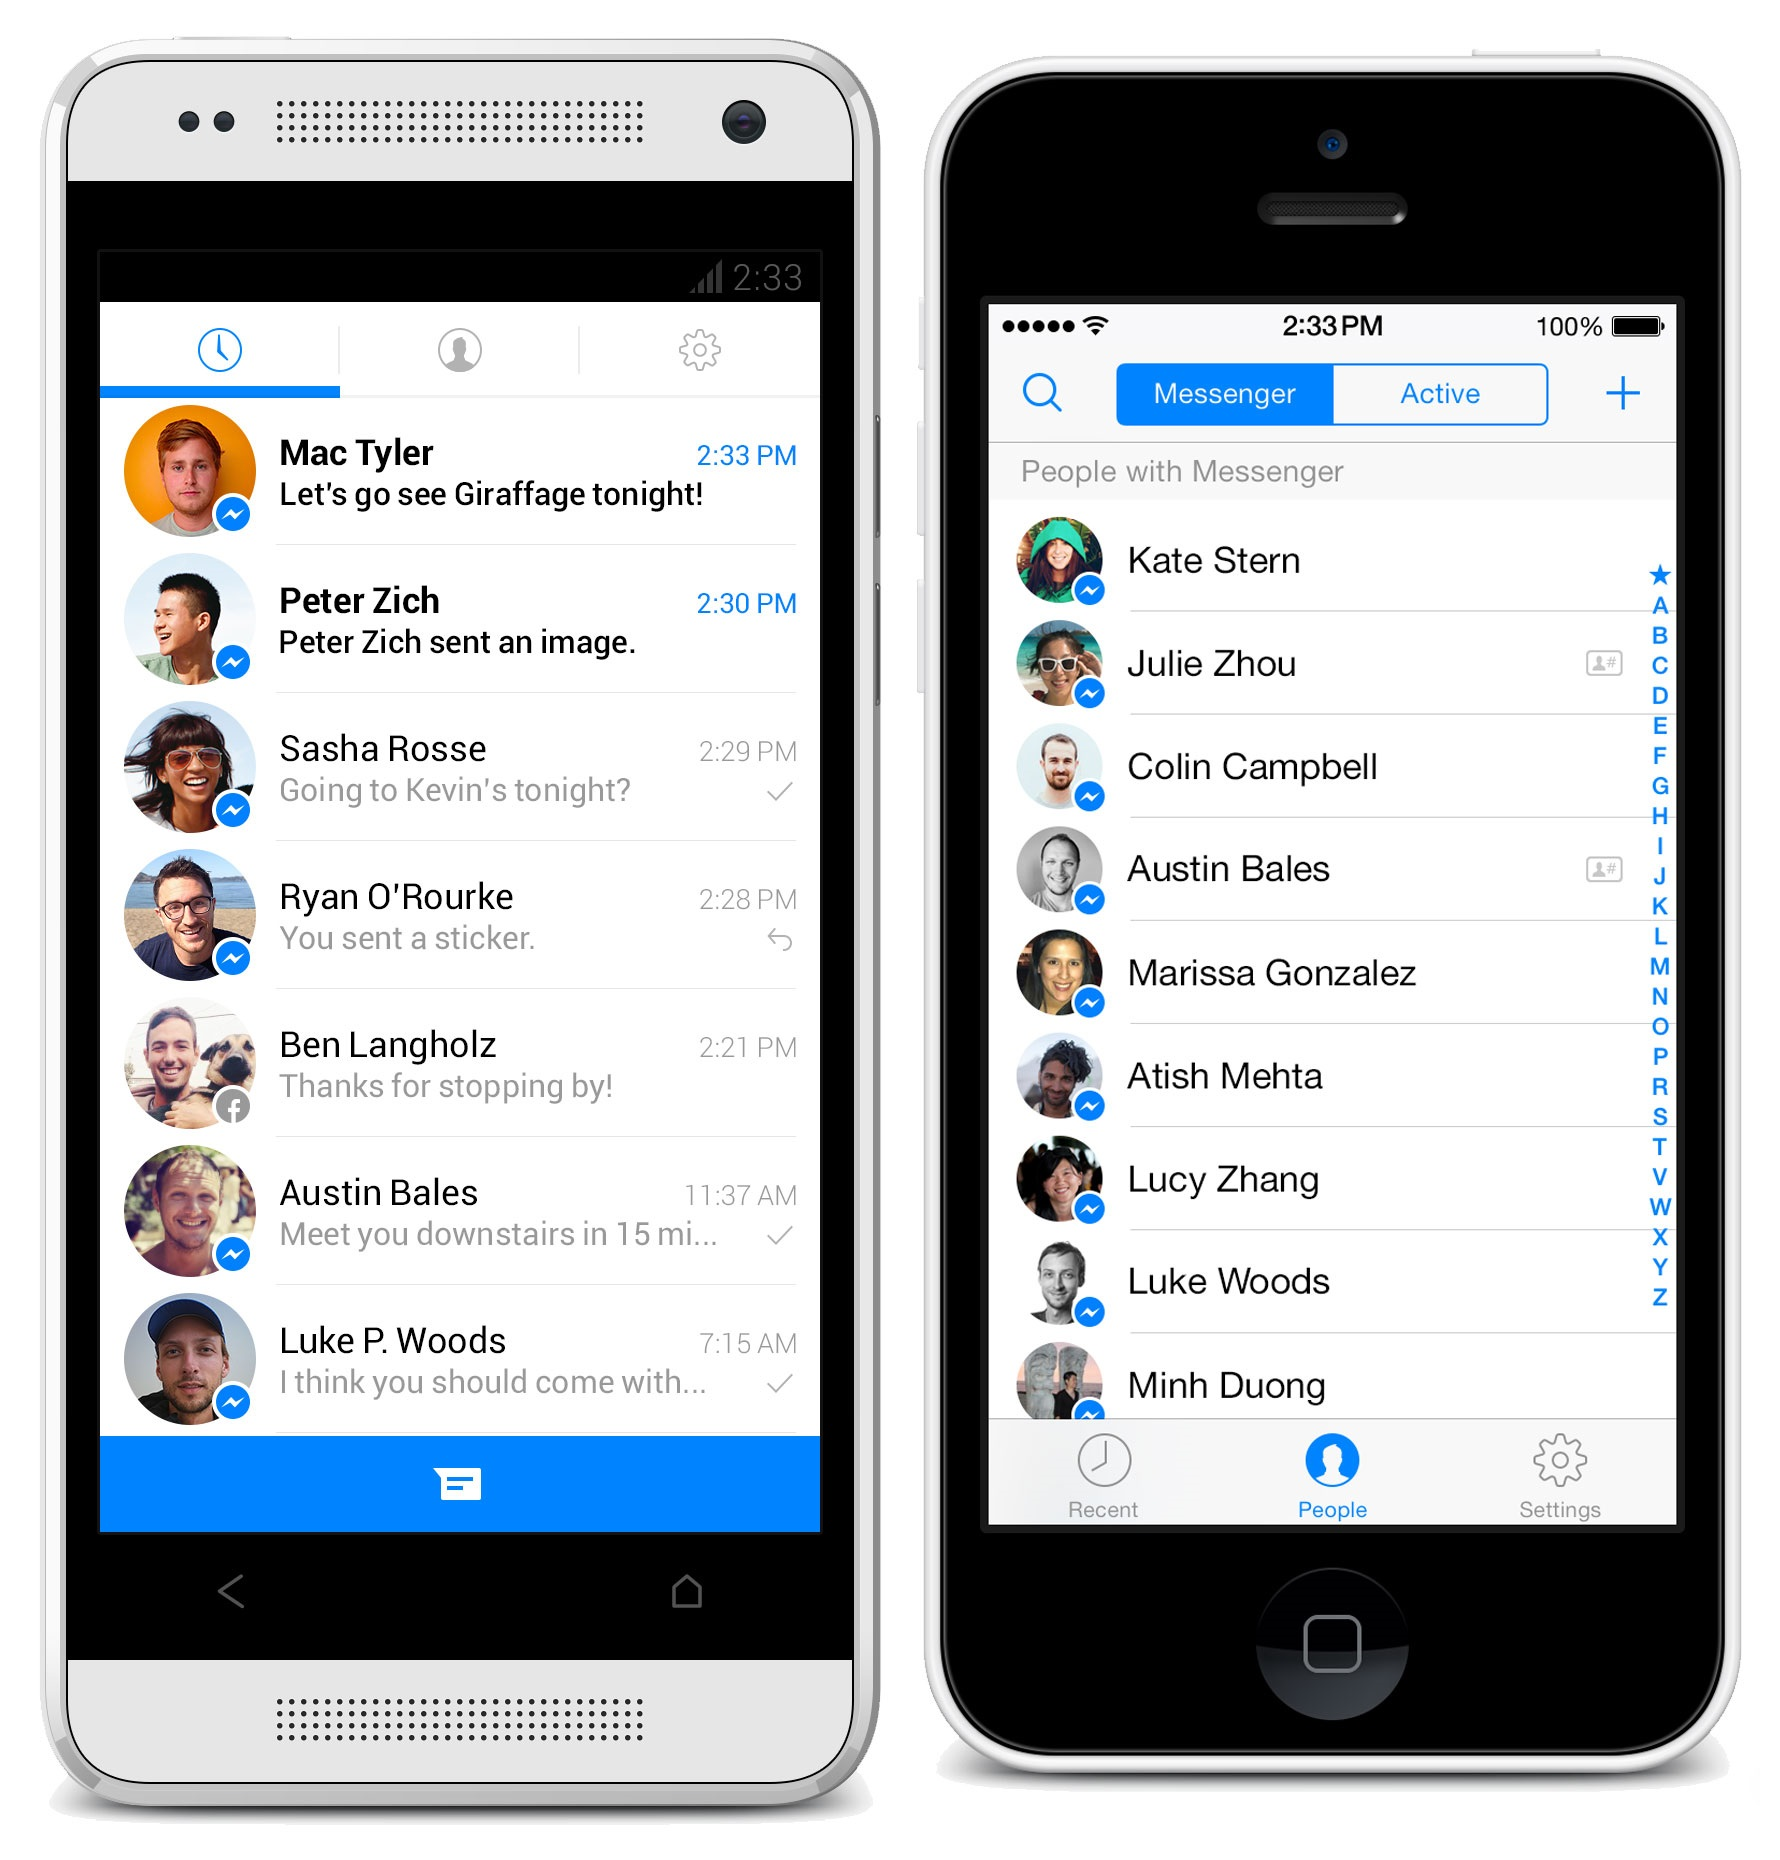
\includegraphics[width=0.22\textwidth]{figures/fb_msg}
  \caption{A composite screenshot of Facebook Messenger}~\label{fig:fbMsg}
\vspace{-20pt}
\end{wrapfigure}

There are also inconsistencies between many similair features. For
example, in the Facebook Messenger app (figure \ref{fig:fbMsg}), when browsing
contacts, the user can move to recent messages and to settings with a context
bar on the bottom. However, when the user is browsing their recent messages, 
the context menu moves to the top and changes slightly in formatting. 

\subsection{Google+}~\label{subsec:google}

Google+ is a relatively new service. It attempts to be an ``all-in-one''
communication platform instead of focusing on the core features. There are far
too many features for organzing that require too much upkeep for the average
user to employ, for example, ``Circles'', which are like contact groups, but
anyone can make then and add people to their Circles, meaning users are
constantly seeing Circles which are likely irrelevant to them. In general, the
Google+ icons and naming conventions don't follow cultural standards.

\begin{wrapfigure}[13]{R}{0.25\textwidth}
  \centering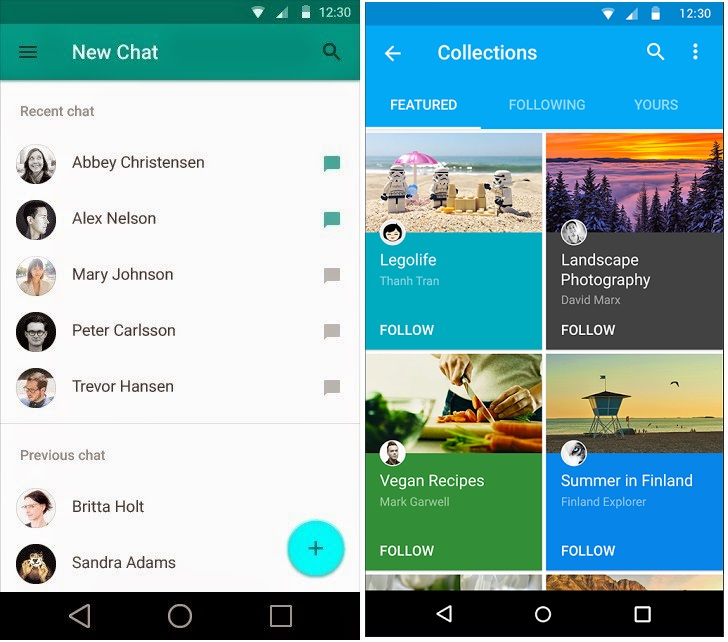
\includegraphics[width=0.22\textwidth]{figures/google_plus}
  \caption{A screenshot of Google Hangouts (left) and Google+ (right)}~\label{fig:google_plus}
\end{wrapfigure}

Google+ does not have a context menu which allows for navigating to different
features. The user must always go back to their homepage/profile to access other
features. Furthermore, the existing context menu is unclear, because the shapes
(triangle, cirlce, square) of the buttons do not indicate what their function
is. In Hangouts (figure \ref{fig:google_plus}), there are two seperate sections
for ``Recent'' and ``Previous'' chat - it is entirely unclear what the
difference is. 

Like Facebook, Google+ forces the user to switch to a completely seperate app
for the chat features, called Google Hangouts. This app has a completely
different design and layout than the Google+ app. 

{\color{red} TODO: two more}

\section{UI design}\label{sec:UI}

\begin{wrapfigure}[11]{r}{0.16\textwidth}%
  \vspace{-33pt}
  \centering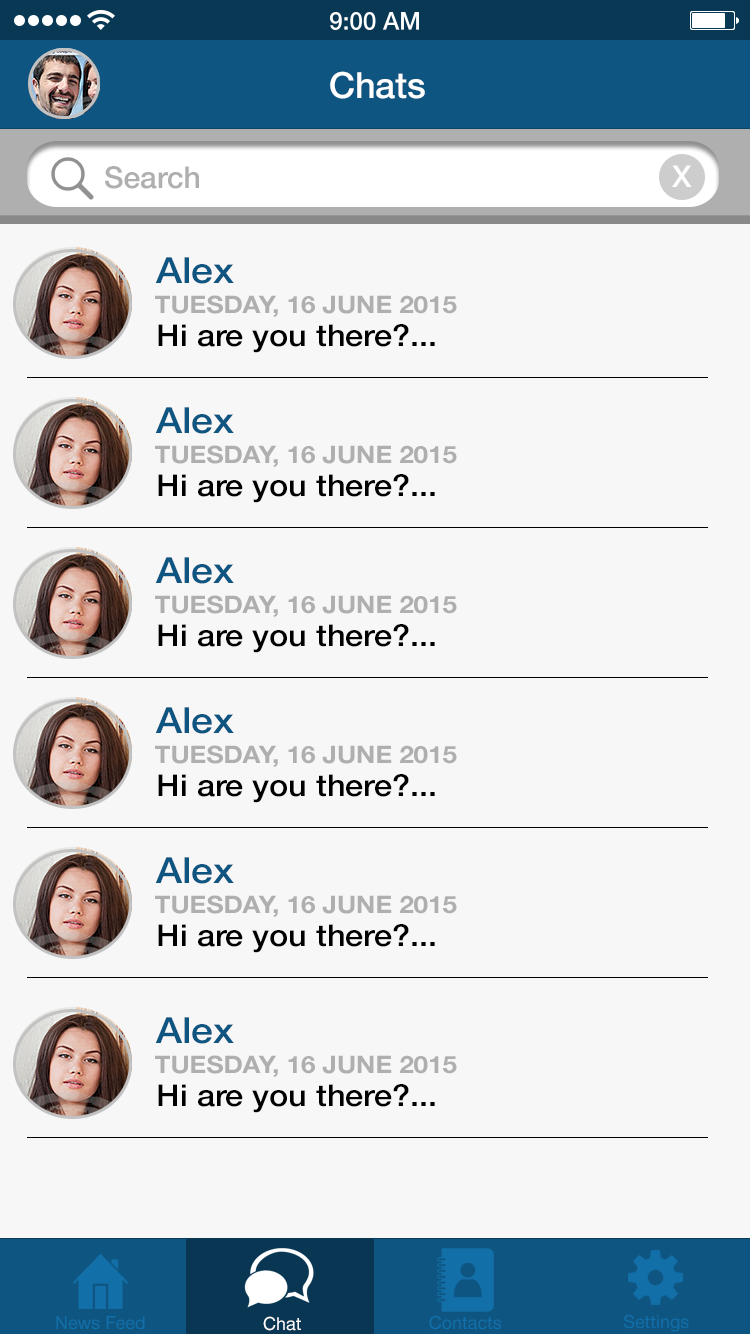
\includegraphics[width=0.13\textwidth]{figures/Chats_EDIT}
  \caption{A mockup of the ``Recent chats'' screen in our UI}~\label{fig:UIchats}
\end{wrapfigure}%

This section details the UI which was designed for our trials. We compare 
selected portions of UI to that of the reviewed softwares. 

Firstly, we integrate the person to person chat features and content browsing
features into a single app (as opposed to multiple apps like Facebook and
Google+), ensuring greater consistency between designs and program logic, and
making the transition between the two features easier.

We strive for high consistency between all contexts. For example, in
almost every screen, you can go to any other top level feature with the context
menu at the bottom.

The context menu only disappears when space on the screen is
extremely valuable; for example, in the actual chat screen, the user wants to
see as much of the conversation as possible. However, seeing all of the news
feed items at once is not as important because the user considers those as
single, independant units. 

\begin{wrapfigure}[14]{r}{0.15\textwidth}
  \vspace{-14pt}
  \centering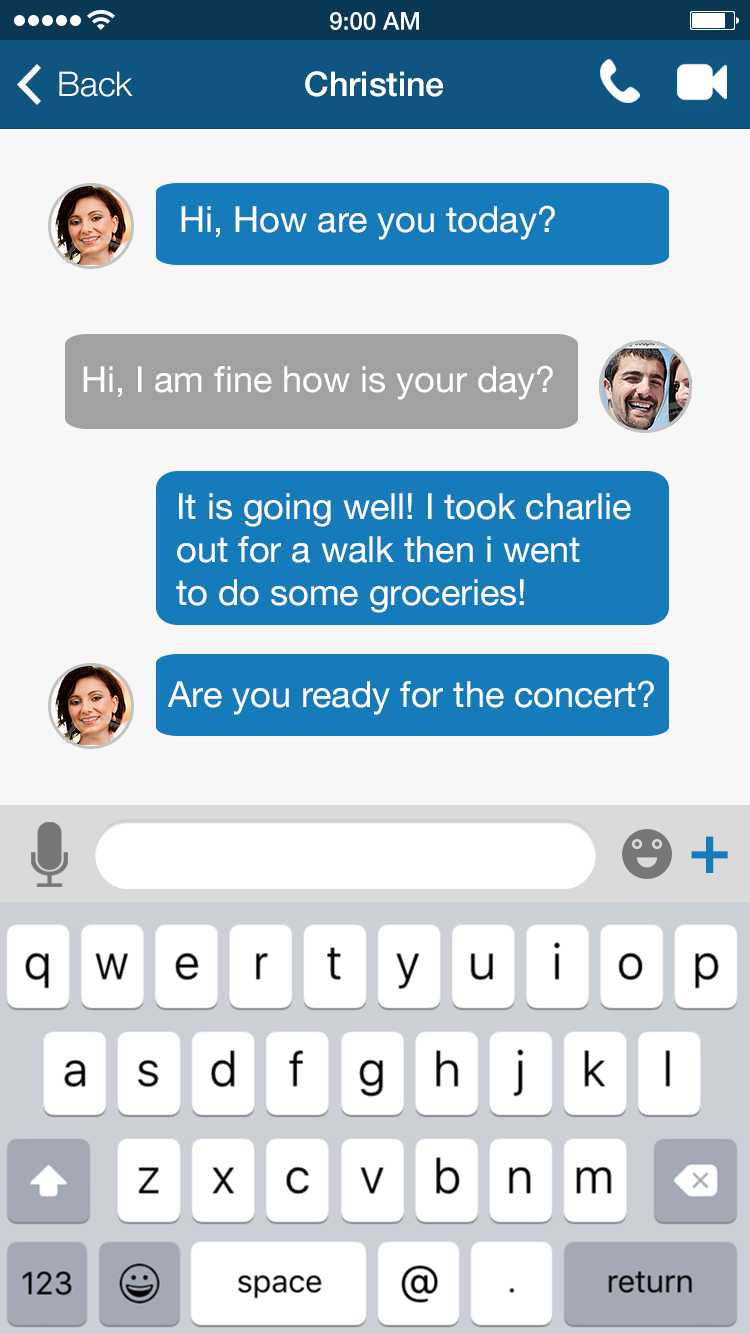
\includegraphics[width=0.13\textwidth]{figures/Regular-convo_02}
  \caption{A mockup of a conversation screen in our UI}~\label{fig:UIconvo}
\end{wrapfigure}

The app uses a great deal of cultural information to make navigation simpler.
Each button has an icon which has a mental mapping to its function, unlike
Google+, which has used arbitrary shapes for many buttons. 

For example, in the conversation screen in figure \ref{fig:UIconvo}, the
text-to-speech button is a microphone, the button which gives users access to
emoticons is a smiley face, the call and video chat buttons are a phone and
video camera, respectively. This mental mapping is very important for users,
especially new users, to learn the application and to quickly get into the flow
of using it; if the initial learning cost is too high, the user will simply give
up.

\begin{wrapfigure}[13]{r}{0.15\textwidth}
  \centering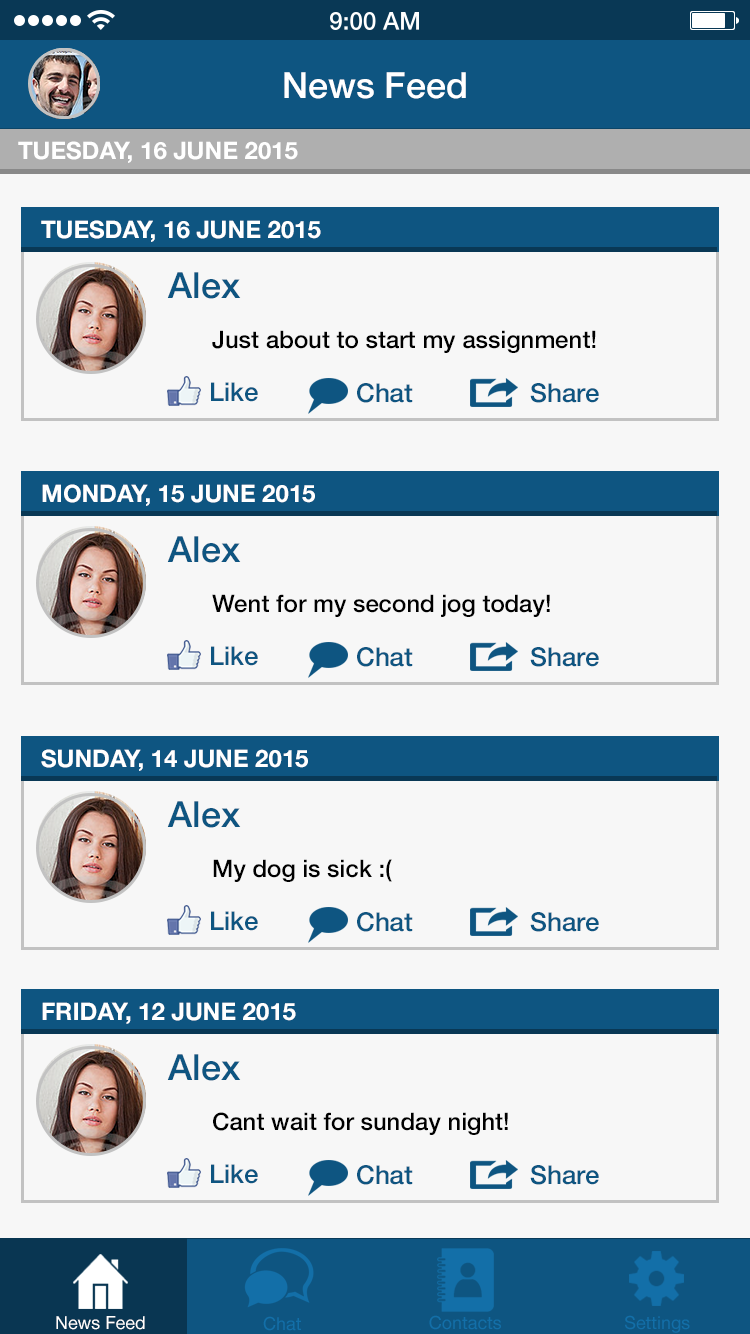
\includegraphics[width=0.13\textwidth]{figures/NewsFeed_EDIT}
  \caption{A mockup of the ``News feed'' screen in our UI}~\label{fig:UInewsfeed}
\end{wrapfigure}

In order to make the application as simple as possible, we limit the complexity of 
each individual screen. Generally, if there are too many UI elements, the user will
start to think that it looks ``cluttered'' or ``messy'', regardless of how well
it is organized, because they are bombarded with an excess of information. 

By limiting
the complexity of each screen, and organizing functions in a highly hierarchal manner, 
we limit the complexity of the UI while preserving ease of use. 

\section{Usability testing}

\noindent This section details our plan to evaluate our new, potentially improved user
interface which was described in the previous section. We describe in detail our
testing procedure, including all involved persons and apparatus.  We describe
our test cases, that is, our actual trials. Finally, we describe how we intend
to evaluate the results of our trials.

 \subsection{Test plan}
 This section details the general test plan, that is, the procedure which
 precedes and follows the actual test cases. The test cases themselves are 
 detailed in the next section. 
  \subsubsection{Participants}
  There are five participants for this trial. Every participant is asked to participate;
  at this time, they are told the following:
    \begin{itemize}
    \item They will be participating in a human-computer interaction study.
    \item It will consist of a trial performed with a personal computer at a desk or table.
    \item After the trial, they will fill out a short questionnaire regarding their experience in the trial. 
    \item It will take no longer than 30 minutes of their time.
    \item They will not be compensated.
    \end{itemize}
  When the participant agrees, they are asked to sign a document attesting to
  the fact that they freely and consciously enter into the study and are aware
  of the conditions.

  \subsubsection{Apparatus}
  The apparatus will consist of the following:
  \begin{itemize}
  \item A laptop computer (belonging to one of the authors).
  \item Paper and writing utencils to record user questionnaire results.
  \end{itemize}

  The only personnel participating in the experiment other than the participants
  are the authors; we act as administrators of the experiment.  

  \subsubsection{Procedure}
  After completing administrative tasks, and when ready to begin, the
  participant is asked to sit at a desk or table at the laptop with our software
  open before them. They are given some task (the specific tasks are detailed in
  the next section) and asked to complete it within the software. The user is
  allowed time to complete the task; after a time limit of 5 minutes, they are
  interrupted.  Each participant is given a sequence of tasks in this
  fashion. The tasks are performed one after the other, with the relative
  ordering of tasks chosen according to a Latin square~\cite[p. 178]{Mackenzie:HCI}. 
  After completion of all tasks, the user is given the questionnaire (which is
  detailed further on) and asked to complete it. Finally, the participant is
  thanked for donating their time.

 \subsection{Test cases}
 All tasks involve interacting with virtual users within the system. These
 ``virtual'' users correspond to some timed events from ``fake'' contacts which
 appear to the user to resemble the actions of some person (like receiving a
 message, seeing a new post appear). Each task has some artificial complexity 
 to simulate a real world thought process, and tasks are randomized where possible
 to ensure they are as representative as possible~\cite[p. 169]{Mackenzie:HCI}. 

  \subsubsection{Send/reply to message} 
  The primary function of an instant messaging software is sending messages. The
  most basic task corresponding to the goal of communicating with one of your
  contacts is to send a message. Messages are always sent for a \emph{reason};
  either the user is replying to a message they received, or they hope to begin
  a conversation with another user. In either case, we must simulate the user
  though process behind sending a message.
  
  To do this, we give the participant a specific task like ``one of your
  contacts has sent you instructions to compute a secret code. You must relay it
  to your friend Bob''. The computation would be something very simple, but
  involves some small amount of thinking. 

  \subsubsection{Find particular activity in newsfeed} 
  Another important feature is browsing the activity of one's contacts. The user
  though process behind this is hard to replicate. We assume that our user
  probably wants to see a particular type of content at a particular time.  For
  example, sometimes the user wants to see pictures of their friends' puppies,
  and sometimes they want to read about the latest drama in their friends'
  lives. 

  To simulate this process, we give the user a task like ``find a post by one of
  your contacts about <some topic>. Respond to this post by
  <commenting/liking/reposting>''. We add some random factors to this task in
  the form of how the participant must ``respond'' to the post, and what topic
  they are searching for. 

  \subsubsection{Create/modify contact} 
  A user obviously will need to create, update, modify and delete their
  contacts.  When a user is doing so, it is because they made a new contact, or
  some old contact's information change. Often, they will have to navigate
  within the application itself to get the new information.

  To simulate this task, we give the user a task like ``your friend Jane posted
  that she got a new phone number. Find her contact and change her phone
  number''. The phone number may be any other personal information, and the 
  ``post'' may also be a message. 

  \subsubsection{Modify a particular setting} 
  Every user will want to customize the software to some degree, even if it is
  just one setting. However, most user don't just play with the settings - if
  something isn't to their liking, they go into the settings with the deliberate 
  purpose of fixing that thing. 

  To simulate the thought process of changing a setting, we give the user a
  task like ``You are unhappy with the font size. Go into the settings and try to 
  change it.'' The font size may be any other feature which is configurable. 

 \subsection{Evaluation criteria} 
  The result of the experiment will be evaluated based on a
  questionnaire~\cite[p. 173]{Mackenzie:HCI} that each participant completes
  upon completion of their tasks, as well as whether or not each task was
  completed in the allotted time (although it is not anticipated that any user
  would fail to do this).

  The questionnaire consists of three sections. The first section asks the participant 
  if they can recall using any similair softwares in the recent past. The participant
  can enter at most three and is strongly encouraged to enter at least one (that is, 
  we don't expect there to be a very high chance of one of our participants never having
  used an instant communication platform) other softwares. They are arbitrarily numbered
  from 1 to 3. Our software is assigned the index 0. 

  The second section consists of a series of questions which ask the participant
  to compare some element of our software to the same element in the softwares
  they listed in section one. The participant is asked to give relative feedback
  to each of the four software (ours, and the three the participant chose) based
  on a series of criteria. The feedback is given using a task load
  index~\cite[p. 174]{Norman:DET}, from 1 (``strongly disagree'') to 5
  (``strongly agree'').

  The criteria in the second section as presented to the participant are as follows:
  \begin{itemize}
  \item Figuring out what buttons perform which function was easy the first time I used the software.
  \item I could easily remember how to access features I had accessed recently. 
  \item I found things where I expected to find them. 
  \item I feel confident using the software after having used it several times. 
  \item The software limited me in what I tried to do.
  \item There was too much pointless information cluttering the screen.
  \item I use (or would use) the majority of the features that the software provides.
  \item I begin to be frustrated with the software quickly. 
  \item The software had a good look and feel to it.
  \end{itemize}

  The third section asks the user to write a short explanation of any other
  successes or deficiencies of the software with which they did the trial.

{\color{red} TODO: trials}

\section{Results}
 \subsection{Findings}
 \subsection{Summary}
\section{Discussion}
 \subsection{Comparative analysis}
 \subsection{Future work}
\section{Conclusion}

% REFERENCES FORMAT
% References must be the same font size as other body text.
\bibliographystyle{SIGCHI-Reference-Format}
\bibliography{sample}

\end{document}

